\chapter{一般图上动态规划的计算}
\label{sec:graph-bag-dp}
\label{chap:general-graph-dp-computation}

上一章构建并核验了计算所需的结构：袋树、选定的根、每个节点的接口与内部变量；有查询时，根袋还包含保留集。本章在这个结构上填写数值表，回答第~\ref{sec:graph-dp-problem}小节提出的几种任务：最小成本及一个最优配置，保留一组变量时的条件最小成本表，可行配置的个数，以及非负权重之积的总和。对每种任务，我们说明输入、输出、递推与正确性，并用算例检验；最后分析这些计算实际需要多少时间和存储。

各任务共用同一套组织方式，第~\ref{sec:graph-dp-assignment-order}节先把它固定下来：每个局部项恰好归入一个容纳其作用域的袋，按后序由叶到根处理，并说明按消元次序计算与沿袋树计算得到同样的中间函数。

第~\ref{sec:graph-dp-min-cost}节处理最小成本。每个袋把本地成本与子袋消息相加，对内部变量取最小，再把结果沿接口交给父袋；取最小时记下达到值的内部取值，根选定最优状态后沿袋树恢复配置。正确性归结为一个不变量：消息等于固定接口后下方全部局部项之和的最小值。第~\ref{sec:graph-dp-retained-min}节保留一组变量，只在根袋中对其余变量取最小，得到以保留变量为索引的表。

第~\ref{sec:graph-dp-semiring}节把相加换成相乘、取最小换成求和，计算可行配置数和加权总和，并说明求和与取最小不能随意交换次序。第~\ref{sec:graph-dp-computation-cost}节把袋与接口换算成实际的表项数，分析时间、存储及二者的取舍。

本章沿用第~\ref{sec:graph-dp-four-cycle}小节的四环算例，并用第~\ref{chap:local-functions-tree-dp}章的三元作用域例子演示消元的逐步过程；两例都可以与枚举结果逐项核对。

% 第13章第1节：局部项归属与求值顺序（局部项的唯一归属、选根与求值顺序、消元与袋树的求值对应）。

\section{局部项归属与求值顺序}
\label{sec:graph-dp-assignment-order}

在填写任何数值之前，要先固定两件事：每个局部项由哪个袋负责，以及各袋按什么顺序计算。这两件事对本章所有任务都相同。先把它们固定下来，既能避免重复计入局部项，也能保证比较两种表示时计算的是同一个对象。

\subsection{局部项的唯一归属}
\label{sec:graph-dp-term-assignment}

计算前先把每个局部函数$\phi_a$归入一个袋$B_{\alpha(a)}$，要求$S_a\subseteq B_{\alpha(a)}$；由引理~\ref{lem:graph-dp-clique-in-bag}，这样的袋总存在。映射$\alpha:A\to T$称为局部项的归属。记归入节点$u$的局部项集合为$A_u=\{a:\alpha(a)=u\}$，它们的和
\begin{equation}
\Phi_u(\bm x_{B_u})=\sum_{a\in A_u}\phi_a(\bm x_{S_a})
\label{eq:graph-dp-bag-cost}
\end{equation}
称为$u$的本地成本。没有局部项归入的袋取$\Phi_u\equiv0$（空和为$0$），但仍保留袋中的变量，因为它们可能需要经过这个袋来保持一致。计数和求和任务把相加换成相乘，空乘积取$1$，第~\ref{sec:graph-dp-semiring}节再说明。

只归入一次是数值正确性的要求。在三元作用域例子的分解$\{1,2,3\}-\{2,3,4\}$中，若另有成对项$\phi_{2,3}(x_2,x_3)$，它可以归入任一袋，但两边各计一次就会求出$F+\phi_{2,3}$的最小值。共享变量可以在多个袋中重复出现，同一个成本项却只能计一次；袋之间的交集本身不对应任何成本。计算前应逐项检查分配清单：无遗漏、无重复、作用域包含于所归的袋。

图~\ref{fig:graph-dp-single-factor-owner}把变量共享与函数归属分开表示。两个袋都保留$2,3$，但$\phi_{2,3}$只沿一条归属箭头进入左袋；把它改归右袋也合法，同时归入两袋则会重复计费。

\begin{figure}[!htb]
  \centering
  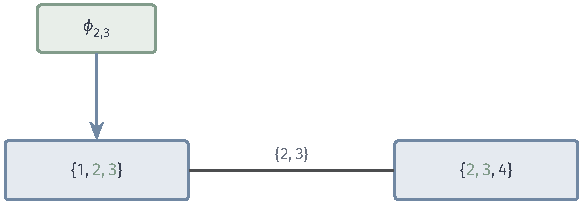
\includegraphics[width=98.651mm]{figures/03-graphs/04-local-functions-and-dynamic-programming/tikz/dp-single-factor-owner/figure.pdf}
  \caption{共享变量不意味着重复计入局部项。两个袋均包含$\phi_{2,3}$的作用域，图中选择左袋作为唯一归属。袋树横边仅表示接口连接，向下的蓝色箭头表示局部项归属，二者含义不同。}
  \label{fig:graph-dp-single-factor-owner}
\end{figure}

\paragraph{消元表示中的归属}
用消元森林表示结构时，归属有一条自然的规则：把$\phi_a$归入$S_a$中最早被消去的变量所对应的袋。第~\ref{sec:graph-dp-clusters-to-decomposition}小节已经说明这个袋包含$S_a$。这条规则恰好对应消元的实际过程：$\phi_a$在它的某个变量第一次被消去时被取出。作用域全在保留集$R$内的局部项（包括作用域为空的常数项）在消元中从不被取出，归入根袋；没有保留集时，常数项可归入任一个根袋。

在四环算例的分解$\{1,2,4\}-\{2,3,4\}$中，$\phi_{1,2}$与$\phi_{1,4}$只能归入$\{1,2,4\}$，$\phi_{2,3}$与$\phi_{3,4}$只能归入$\{2,3,4\}$。按次序$(1,2,3,4)$的消元森林来看，$\phi_{3,4}$本应归入$B_3=\{3,4\}$，这个袋并入$\{2,3,4\}$后归属随之并入。

三元作用域例子的分解中，$\phi_A$只能归入$\{1,2,3\}$，$\phi_B$只能归入$\{2,3,4\}$。

\subsection{选根与求值顺序}
\label{sec:graph-dp-root-order}

给已核验的袋树选根$r$，确定每个非根节点$u$的父节点$p(u)$、子节点集合$\operatorname{ch}(u)$、接口$S_u=B_u\cap B_{p(u)}$与内部变量$I_u=B_u\setminus S_u$（第~\ref{sec:graph-dp-interface-internal}小节）。查询任务使用第~\ref{sec:graph-dp-query-structure}小节保证覆盖保留集$R$的根袋。

求值按袋树的一个后序进行：先处理全部子节点，再处理父节点，最后处理根。每个非根节点只用到子节点交来的表，处理完后把一张以$\bm x_{S_u}$为索引的表交给父节点。后序可以由一次深度优先遍历的完成次序得到，它与根、父节点一样只规定处理次序，在运行中不变。需要恢复配置时，再按前序（后序的逆序，父节点总在子节点之前）走一遍。

原始图不连通时，各分量的袋树之间只有空接口的边相连。沿空接口传递的表只有一项，是一个数：最小成本任务中它是那个分量的最小成本，计数和求和任务中它是那个分量的总数或总和。根把收到的这些数与本分量的结果组合起来，组合方式随任务而定，在各任务中分别说明。

\paragraph{表的存储与对齐}
本地成本、消息和回溯表都是以一组变量为索引的稠密表。为每张表固定变量的排列（例如按编号），各取值按字典序存放，即$(x_{j_1},\ldots,x_{j_k})$像多位数一样以最后一个变量为最低位递增。于是一组取值的位置可以按混合进制直接算出，读取一项按常数时间计；本部分例子中的表都按这种次序列出，例如作用域为$\{2,4\}$的表依次对应$(x_2,x_4)=(0,0),(0,1),(1,0),(1,1)$。

计算时要在袋$B_u$的一组取值$\bm x_{B_u}$上读取$\phi_a(\bm x_{S_a})$或子节点的消息，即从$\bm x_{B_u}$中挑出$S_a$或$S_c$的那几个分量，再算它们在小表中的位置。各变量在$B_u$中的位置事先记下，每次读取就只需几次乘加。接口上的“对齐”指的正是这一步：发送方和接收方按同一组接口变量、同一排列存取消息。

\subsection{消元与袋树的求值对应}
\label{sec:graph-dp-elimination-message-correspondence}

第~\ref{sec:graph-dp-function-message-correspondence}小节在结构上对应了消元簇与袋、剩余作用域与接口。现在在数值上验证这一对应。沿袋树计算时，非根节点$u$先把本地成本与子节点的消息相加，得到
\[
g_u(\bm x_{B_u})=\Phi_u(\bm x_{B_u})+\sum_{c\in\operatorname{ch}(u)}m_{c\to u}(\bm x_{S_c}),
\]
再对内部变量取最小，得到发往父节点的消息
\[
m_{u\to p(u)}(\bm x_{S_u})=\min_{\bm x_{I_u}}g_u(\bm x_{B_u}).
\]
第~\ref{sec:graph-dp-min-cost}节逐项解释这两步。

\begin{theorem}[消元中间函数等于袋消息]
\label{thm:graph-dp-elimination-equals-messages}
设$\pi=(v_1,\ldots,v_k)$是$V\setminus R$的消元次序，袋树由算法~\ref{alg:graph-dp-order-to-decomposition}得到并以消元森林的根（有保留集时为$B_R$）为根，局部项按“作用域中最早被消去的变量”归属，作用域含于$R$的项归入根袋。则按次序消元时，第$i$步取出的函数恰为$\{\phi_a:a\in A_{B_i}\}$与$\{\psi_j:B_j\text{的父袋是}B_i\}$，并且$\psi_i=m_{B_i\to p(B_i)}$。
\end{theorem}

\begin{proof}
消元过程中，当前函数集合里的每个函数，作用域只含尚未消去的变量；它在作用域中第一个变量被消去时被取出，此前一直不动。原始局部项$\phi_a$因此在$S_a$中最早被消去的变量那一步被取出，这正是它的归属。中间函数$\psi_j$的作用域是$S_j$，它在$S_j$中最早被消去的变量那一步被取出，这正是$B_j$的父袋；若$S_j\subseteq R$，它从不被取出，最后留在根袋。这就证明了第一个断言。

再对$i$归纳证明$\psi_i=m_{B_i\to p(B_i)}$。第$i$步取出的函数之和为$\Phi_{B_i}$加上各子袋的$\psi_j$；由归纳假设，后者等于子袋发来的消息，所以这个和就是$g_{B_i}$。$B_i$的内部变量只有$v_i$（第~\ref{sec:graph-dp-function-message-correspondence}小节），所以式~\eqref{eq:graph-dp-elimination-step}的$\psi_i=\min_{x_{v_i}}g_{B_i}$正是消息$m_{B_i\to p(B_i)}$。
\end{proof}

证明只用到“先把取出的函数组合起来，再对一个变量汇总”这一结构，没有用到取最小或相加的具体性质；把它们换成求和与相乘，同样的对应在第~\ref{sec:graph-dp-semiring}节的计数和求和中成立。

\paragraph{合并袋与一次处理多个内部变量}
实际使用的袋树常常把消元森林中相邻的袋合并，例如四环算例把$\{2,3,4\},\{3,4\},\{4\}$并成一个根袋。合并后的袋一次处理多个内部变量：沿袋树的消息是对这些变量同时取最小，而按次序消元则是逐个取最小。由式~\eqref{eq:graph-dp-min-rules}的第一条，对几个变量同时取最小等于逐个取最小，所以合并改变的只是中间表，不改变发往父袋的消息和最终结果。更一般的情形，即任意合法分解、任意满足容纳条件的归属，由第~\ref{sec:graph-dp-min-cost-correctness}小节的不变量统一证明。

\paragraph{例子}
三元作用域例子按次序$(1,4,2,3)$消元，得到的袋树是$\{1,2,3\}\to\{2,3\}\leftarrow\{2,3,4\}$、$\{2,3\}\to\{3\}$，以$\{3\}$为根。各条消息恰好是第~\ref{sec:graph-dp-min-cost-recovery}小节表~\ref{tab:graph-dp-elimination-trace}中的$\psi_1,\psi_4$与消去$x_2$得到的新函数。

第~\ref{sec:graph-dp-tree-messages}小节的树上递推也是这样的特例：对依赖树选定根，以$\{u,p(u)\}$为袋（第~\ref{sec:graph-tree-decomposition}小节宽度为$1$的分解），把$\phi_u$和$\phi_{u,p(u)}$归入这个袋（根的一元项归入任一个含根的袋），接口就是单个变量$p(u)$，袋消息退化为顶点之间的消息。

% 第13章第2节：最小成本（合并本地成本与子消息、消去接口外变量、根袋求值、最优配置的记录与恢复、计算正确性、四环算例与边界检验）。

\section{最小成本}
\label{sec:graph-dp-min-cost}

本节的输入是各变量的有限状态集合、局部成本表（取值于$\mathbb R\cup\{+\infty\}$），以及上一节固定的袋树、根、后序和局部项归属；输出是最小成本$F^\star=\min_{\bm x}F(\bm x)$，并在$F^\star$有限时给出一个达到它的配置，在$F^\star=+\infty$时报告没有可行配置。数值递推、达到值的记录、回溯、正确性与检验在本节一起展开。

\subsection{合并本地成本与子消息}
\label{sec:graph-dp-bag-merge}

处理节点$u$时，它的子节点都已处理完，各自交来一张以接口为索引的消息表$m_{c\to u}(\bm x_{S_c})$，$c\in\operatorname{ch}(u)$。第一步是把本地成本与这些消息按同一个袋配置读取并相加：
\begin{equation}
g_u(\bm x_{B_u})=\Phi_u(\bm x_{B_u})+\sum_{c\in\operatorname{ch}(u)}m_{c\to u}(\bm x_{S_c}).
\label{eq:graph-dp-bag-merge}
\end{equation}
由于$S_c\subseteq B_u$、$S_a\subseteq B_u$（$a\in A_u$），右端每一项都只读取$\bm x_{B_u}$的一部分分量，按第~\ref{sec:graph-dp-root-order}小节的对齐方式取出即可。$g_u$的含义是：袋内变量取定$\bm x_{B_u}$时，$u$本地的成本加上各子节点下方最好能做到的成本。

叶节点没有子消息，求和为空，$g_u=\Phi_u$；没有局部项归入的节点$\Phi_u\equiv0$，$g_u$只由子消息组成。两种空和都取$0$，每项原始成本仍恰好计入一次：它在自己所归的节点计入$\Phi$，此后只以消息的形式向上传递。

在四环算例中，叶节点$\{1,2,4\}$的合并结果是
\[
g(x_1,x_2,x_4)=\phi_{1,2}(x_1,x_2)+\phi_{1,4}(x_1,x_4);
\]
根$\{2,3,4\}$的合并结果是$\phi_{2,3}+\phi_{3,4}$加上叶节点交来的消息。

\subsection{消去接口外变量}
\label{sec:graph-dp-bag-idea}
\label{sec:graph-dp-elimination-idea}

第二步对内部变量取最小。记父节点为$p=p(u)$、接口为$S_u=B_u\cap B_p$，从$u$发往$p$的消息是
\begin{equation}
m_{u\to p}(\bm x_{S_u})=\min_{\bm x_{I_u}}g_u(\bm x_{S_u},\bm x_{I_u}),\qquad I_u=B_u\setminus S_u .
\label{eq:graph-dp-bag-message}
\end{equation}
这与式~\eqref{eq:graph-dp-tree-message}的结构相同，只是被汇总的不再是单个变量，而是袋内全部非接口变量。

可以把每个袋想成一个只看得见袋内变量的计算者。$u$向父节点汇报的是：“若接口取这组值，我这一侧最好能做到多少成本。”父节点不需要知道$u$一侧的其他变量取什么，因为由第~\ref{sec:graph-dp-interface-separation}小节的分隔性质，这些变量不会在父节点一侧再出现，它们只需在$u$一侧选好即可。“$u$一侧最好能做到多少”这一含义在第~\ref{sec:graph-dp-min-cost-correctness}小节证明。

\paragraph{两种退化情形}
接口为空时，消息只有一项，是一个数，但仍须对全部内部配置取最小，不能省去这一步。没有内部变量时（$B_u\subseteq B_p$），式~\eqref{eq:graph-dp-bag-message}中没有可取最小的变量，消息就是$g_u$本身，作为$\bm x_{S_u}=\bm x_{B_u}$的函数原样交给父节点。

\paragraph{数值消元更新}
内部变量只有一个时，式~\eqref{eq:graph-dp-bag-message}就是式~\eqref{eq:graph-dp-elimination-step}的数值消元更新：消元森林中第$i$个袋的内部变量是$v_i$，消息就是$\psi_i$（定理~\ref{thm:graph-dp-elimination-equals-messages}）。

在三元作用域例子中消去$x_1$：只有$\phi_A$含$1$，$S_1=\{2,3\}$。对$(x_2,x_3)=(0,0),(0,1),(1,0),(1,1)$，分别比较$x_1=0,1$两行，得到
\[
\psi_1(x_2,x_3)=\bigl(\min(1,0),\ \min(0,2),\ \min(2,1),\ \min(+\infty,2)\bigr)=(0,\,0,\,1,\,2),
\]
达到最小值的$x_1$依次为$1,0,1,1$。消元后的函数集合是$\{\psi_1,\phi_B\}$。

这一步没有改变剩余变量的最优成本，可以逐项核对。

例如取$(x_2,x_3,x_4)=(1,0,1)$，原问题对$x_1$求最小值为
\[
\begin{aligned}
&\min\bigl(\phi_A(0,1,0)+\phi_B(1,0,1),\ \phi_A(1,1,0)+\phi_B(1,0,1)\bigr)\\
&\qquad=\min(2,1)=1.
\end{aligned}
\]
新集合给出
\[
\psi_1(1,0)+\phi_B(1,0,1)=1+0=1,
\]
两者相同。第~\ref{sec:graph-dp-min-cost-correctness}小节证明这种一致对每个剩余配置、每一步消元都成立。

\subsection{根袋求值}
\label{sec:graph-dp-root-evaluation}

全部非根节点处理完后，根$r$按式~\eqref{eq:graph-dp-bag-merge}合并本地成本与全部子消息，得到$g_r(\bm x_{B_r})$。根的内部变量是整个$B_r$，于是
\begin{equation}
F^\star=\min_{\bm x_{B_r}}g_r(\bm x_{B_r}).
\label{eq:graph-dp-root-min}
\end{equation}
用消元表示时，这对应消去根袋中剩余的变量，剩下的常数就是最小成本。

原始图不连通时，其他分量的根经空接口交来的消息都是标量，即各分量的最小成本；它们作为常数加进$g_r$，所以$F^\star$等于各分量最小成本之和。这与式~\eqref{eq:graph-dp-min-rules}后的第三条规则一致：互不相交的变量组可以分别取最小再相加。

若$F^\star=+\infty$，报告没有可行配置，不做恢复；若$F^\star$有限，进入下一小节的恢复步骤。

\subsection{最优配置的记录与恢复}
\label{sec:graph-dp-min-cost-recovery}
\label{sec:graph-dp-bag-algorithm}
\label{sec:graph-dp-elimination-algorithm}

与链和树上一样，取最小值丢掉了达到者，所以计算消息时要同时记录达到值。对每个接口取值$\bm x_{S_u}$，若$m_{u\to p}(\bm x_{S_u})$有限，记下一个达到最小值的内部取值$b_u(\bm x_{S_u})\in\prod_{i\in I_u}\mathcal X_i$，称为回溯表；并列时按固定规则选取，本部分约定取字典序最小者。若$m_{u\to p}(\bm x_{S_u})=+\infty$，这个接口取值下没有可行的内部取值，不生成记录。根处同样记下$g_r$的一个最小点。

恢复按前序进行：
\begin{itemize}
  \item 根：取$g_r$的最小点（并列时取字典序最小者）作为$\bm x^\star_{B_r}$；
  \item 非根节点：轮到$u$时，它的接口变量都在父袋中，父节点已经处理，所以$\bm x^\star_{S_u}$已经取定；查$b_u(\bm x^\star_{S_u})$，给内部变量$\bm x^\star_{I_u}$赋值。
\end{itemize}
每个变量恰在一个节点作内部变量（引理~\ref{lem:graph-dp-unique-internal}），所以恰被赋值一次，在它出现的所有袋中取同一个值。用消元表示时，按前序恢复就是按消元的逆序回溯：轮到$v_i$时，$S_i$中的变量都比$v_i$晚消去，在逆序中已经取定。

\paragraph{两种表示的算法}
按消元次序直接计算时，每个函数存为一个作用域和一张稠密表，并为每个变量维护一张索引，列出当前作用域含它的函数，消去$x_i$时据此直接取出$\mathcal F_i$，不必扫描全部函数。算法维护当前函数集合（初值为全部局部函数）、已消去的变量集合和各步的回溯表。

\begin{algorithm}[变量消元求最小成本]
\label{alg:graph-dp-variable-elimination}
输入：有限状态集合、局部函数表、一个消元次序。输出：最小成本，以及一个最优配置或“不可行”。
\begin{enumerate}
  \item 按次序取下一个变量$x_i$，由变量索引取出当前全部含$i$的函数$\mathcal F_i$，确定$S_i$。
  \item 对$\bm x_{S_i}$的每个取值，枚举$x_i$的全部状态，按式~\eqref{eq:graph-dp-elimination-step}求$\psi_i$；同时把达到最小值的$x_i$（并列时取编号最小者）记入回溯表$b_i(\bm x_{S_i})$。
  \item 用$\psi_i$替换$\mathcal F_i$，同步更新$S_i$中各变量的索引；重复直到变量全部消去，剩下的常数之和即最小成本。
  \item 若最小成本为$+\infty$，报告不可行；否则按消元的逆序依次令$x_i=b_i(\bm x_{S_i})$。
\end{enumerate}
\end{algorithm}

\begin{algorithm}[树分解上的最小成本动态规划]
\label{alg:graph-dp-bag-dp}
输入：局部函数表，原始图的已核验树分解。输出：最小成本，以及一个最优配置或“不可行”。
\begin{enumerate}
  \item 把每个局部函数归入一个包含其作用域的袋，按式~\eqref{eq:graph-dp-bag-cost}计算各袋本地成本$\Phi_u$。
  \item 选根节点$r$，求出每个节点的父节点、接口、内部变量和一个后序。
  \item 按后序处理每个非根节点$u$：按式~\eqref{eq:graph-dp-bag-merge}合并得$g_u$；对接口$S_u$的每种取值，枚举$I_u$的全部取值，按式~\eqref{eq:graph-dp-bag-message}计算$m_{u\to p(u)}$，并把达到最小值的内部取值记入$b_u$。
  \item 合并得$g_r$，按式~\eqref{eq:graph-dp-root-min}计算最小成本；若为$+\infty$，报告不可行并停止。
  \item 取$g_r$的最小点为根袋变量赋值；按前序处理每个非根节点$u$，查$b_u$为$I_u$赋值。
\end{enumerate}
\end{algorithm}

\paragraph{消元的执行过程}
在三元作用域例子上按次序$(1,4,2,3)$执行算法~\ref{alg:graph-dp-variable-elimination}。下面逐步比较更新前后的函数集合，最后用表~\ref{tab:graph-dp-elimination-trace}汇总数值。

消去$x_1$：如上一小节，$\mathcal F_1=\{\phi_A\}$，$S_1=\{2,3\}$，$\psi_1=(0,0,1,2)$，$b_1=(1,0,1,1)$。函数集合变为$\{\psi_1,\phi_B\}$。
\begin{BookInlineFigure}
  \centering
  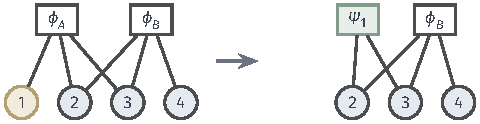
\includegraphics[width=81.284mm]{figures/03-graphs/04-local-functions-and-dynamic-programming/tikz/reading-steps/eliminate-x1.pdf}
  \caption{消去$x_1$：把读取它的$\phi_A$替换为$\psi_1(x_2,x_3)$，$\phi_B$不变。圆点为变量，方块为函数，连线表示读取关系；左侧黄色变量被汇总，右侧绿色方块是新函数。}
  \label{fig:graph-dp-elimination-trace}
\end{BookInlineFigure}

消去$x_4$：只有$\phi_B$含$4$，$S_4=\{2,3\}$。对$(x_2,x_3)$的四种取值比较$x_4=0,1$，得到
  \[
  \psi_4=\bigl(\min(2,1),\ \min(0,+\infty),\ \min(+\infty,0),\ \min(1,2)\bigr)=(1,0,0,1),
  \]
  回溯表$b_4=(1,0,1,0)$。函数集合变为$\{\psi_1,\psi_4\}$。
\begin{BookInlineFigure}
  \centering
  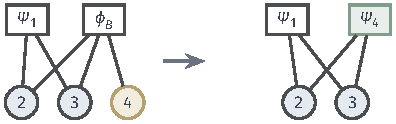
\includegraphics[width=67.035mm]{figures/03-graphs/04-local-functions-and-dynamic-programming/tikz/reading-steps/eliminate-x4.pdf}
  \caption{消去$x_4$：$\phi_B$被$\psi_4(x_2,x_3)$替换。此时两个函数只共享接口变量$x_2,x_3$。}
  \label{fig:graph-dp-elimination-trace-x4}
\end{BookInlineFigure}

消去$x_2$：$\psi_1$和$\psi_4$都含$2$，要先相加再对$x_2$取最小，$S_2=\{3\}$。$x_3=0$时两个候选为
  \[
  \psi_1(0,0)+\psi_4(0,0)=1,\qquad \psi_1(1,0)+\psi_4(1,0)=1,
  \]
  二者并列，按约定取$x_2=0$。$x_3=1$时候选为$0+0=0$与$2+1=3$，取$x_2=0$。新函数记为$\psi_2'=(1,0)$，以区别于第~\ref{sec:graph-dp-fill-in}小节先消$x_2$时的$\psi_2$；$b_2=(0,0)$。
\begin{BookInlineFigure}
  \centering
  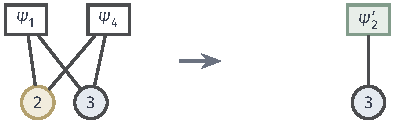
\includegraphics[width=66.784mm]{figures/03-graphs/04-local-functions-and-dynamic-programming/tikz/reading-steps/eliminate-x2.pdf}
  \caption{消去$x_2$：先把同一$(x_2,x_3)$下的$\psi_1$与$\psi_4$相加，再对$x_2$取最小。两项共同被一元函数$\psi_2'(x_3)$替换。}
  \label{fig:graph-dp-elimination-trace-x2}
\end{BookInlineFigure}

消去$x_3$：只剩$\psi_2'$，$S_3=\varnothing$，$\min(1,0)=0$在$x_3=1$处达到，$b_3=1$。函数集合只剩常数$0$，即最小成本。
\begin{BookInlineFigure}
  \centering
  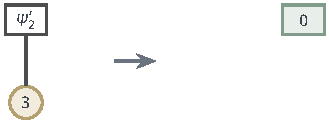
\includegraphics[width=55.785mm]{figures/03-graphs/04-local-functions-and-dynamic-programming/tikz/reading-steps/eliminate-x3.pdf}
  \caption{消去$x_3$：对最后的一元函数$\psi_2'$取最小，得到常数$0$。新函数已无变量，因而右侧没有连线。}
  \label{fig:graph-dp-elimination-trace-x3}
\end{BookInlineFigure}

最小成本有限，按逆序$3,2,4,1$回溯：
\[
\begin{gathered}
x_3=b_3=1,\qquad x_2=b_2(x_3{=}1)=0,\\
x_4=b_4(x_2{=}0,x_3{=}1)=0,\qquad x_1=b_1(x_2{=}0,x_3{=}1)=0.
\end{gathered}
\]

\begin{BookInlineFigure}
  \centering
  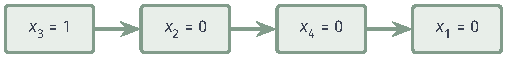
\includegraphics[width=85.785mm]{figures/03-graphs/04-local-functions-and-dynamic-programming/tikz/reading-steps/elimination-recovery.pdf}
  \caption{按消元的逆序查回溯表。先确定$x_3$，再用已知接口值依次读取$b_2,b_4,b_1$，恢复$(x_1,x_2,x_3,x_4)=(0,0,1,0)$。}
  \label{fig:graph-dp-elimination-trace-recovery}
\end{BookInlineFigure}

恢复的配置为$(0,0,1,0)$，代回表~\ref{tab:graph-dp-ternary-tables}得
\[
\phi_A(0,0,1)+\phi_B(0,1,0)=0+0=0,
\]
与枚举结果一致。

\begin{table}[!htb]
  \centering
  \small
  \begin{tabular}{@{}cccccc@{}}
    \toprule
    消去 & 取出$\mathcal F_i$ & $S_i$ & 新函数$\psi_i$ & 回溯表$b_i$ & 消元后的$\mathcal F$\\
    \midrule
    $x_1$ & $\phi_A$ & $\{2,3\}$ & $(0,0,1,2)$ & $(1,0,1,1)$ & $\{\psi_1,\phi_B\}$\\
    $x_4$ & $\phi_B$ & $\{2,3\}$ & $(1,0,0,1)$ & $(1,0,1,0)$ & $\{\psi_1,\psi_4\}$\\
    $x_2$ & $\psi_1,\psi_4$ & $\{3\}$ & $(1,0)$ & $(0,0)$ & $\{\psi_2'\}$\\
    $x_3$ & $\psi_2'$ & $\varnothing$ & $0$ & $1$ & $\{0\}$\\
    \bottomrule
  \end{tabular}
  \caption{按次序$(1,4,2,3)$对三元作用域例子消元。新函数与回溯表的取值按剩余变量的字典序列出：作用域为$\{2,3\}$时依次对应$(x_2,x_3)=(0,0),(0,1),(1,0),(1,1)$，作用域为$\{3\}$时对应$x_3=0,1$。}
  \label{tab:graph-dp-elimination-trace}
\end{table}


\paragraph{袋树上的执行过程}
同一个例子也可以直接在两个袋$B_s=\{1,2,3\}$、$B_t=\{2,3,4\}$上执行算法~\ref{alg:graph-dp-bag-dp}，取$t$为根，后序为$s,t$。本地成本为$\Phi_s=\phi_A$、$\Phi_t=\phi_B$。

$s$是叶节点，没有子消息，内部变量只有$x_1$，所以
\[
m_{s\to t}(x_2,x_3)=\min_{x_1}\phi_A(x_1,x_2,x_3).
\]
图~\ref{fig:graph-dp-bag-message-table}逐行列出了这张四项表：接口取值为$00,01,10,11$时，消息值依次为$0,0,1,2$，达到最小值的$x_1$依次为$1,0,1,1$。它与消去$x_1$得到的$\psi_1$相同。

$x_1$已经被汇总，不再出现在表中；$x_2,x_3$作为接口仍然显式保留，根袋读取这张表时要按同样的$(x_2,x_3)$取值对齐。

根处合并得$g_t=\phi_B+m_{s\to t}$，按$(x_2,x_3,x_4)$的字典序依次为
\[
g_t=(2,\,1,\,0,\,+\infty,\,+\infty,\,1,\,3,\,4),
\]
最小值$0$在$(0,1,0)$处达到。

回溯时根取$(x_2,x_3,x_4)=(0,1,0)$，查叶节点的回溯表得$b_s(0,1)=0$，即$x_1=0$。恢复的配置$(0,0,1,0)$与枚举和消元的结果相同。

\begin{figure}[!htb]
  \centering
  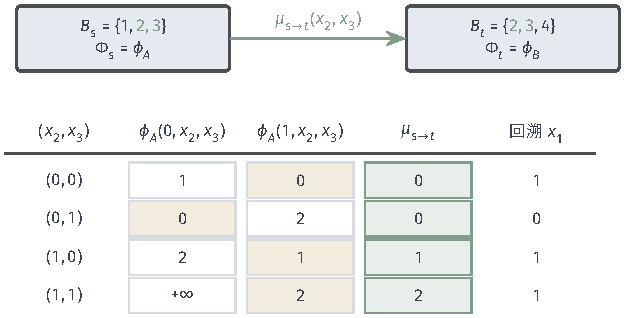
\includegraphics[width=105.650mm]{figures/01-basic-mathematics/04-graphs/tikz/c5-bag-message-table/figure.pdf}
  \caption{两袋之间的消息。左袋$B_s=\{1,2,3\}$只含$\phi_A$，右袋$B_t=\{2,3,4\}$只含$\phi_B$，接口为$\{2,3\}$（绿色）。下方表格对接口的每种取值比较$x_1=0,1$两个候选，取较小者作为消息值，黄色格是被选中的候选；绿色列是消息值，最后一列是回溯表。根袋$B_t$把消息与$\phi_B$相加后对$x_2,x_3,x_4$取最小，得到最优值$0$。}
  \label{fig:graph-dp-bag-message-table}
\end{figure}

\subsection{计算正确性}
\label{sec:graph-dp-min-cost-correctness}
\label{sec:graph-dp-bag-analysis}
\label{sec:graph-dp-elimination-analysis}

\paragraph{消息的不变量}
正确性归结为一个不变量：每条消息等于固定接口后，下方全部局部项之和的最小值。对非根节点$u$，记$D_u$为$u$及其全部后代组成的节点集合，$V_{D_u}=\bigcup_{t\in D_u}B_t$为这些袋中出现的变量，$A_{D_u}=\bigcup_{t\in D_u}A_t$为归入这些节点的局部项。

\begin{theorem}[袋消息的含义]
\label{thm:graph-dp-bag-message}
设$(\mathcal T,\{B_t\}_{t\in T})$是原始图的树分解，以$r$为根，每个局部函数恰好归入一个包含其作用域的袋。则对每个非根节点$u$和每个接口取值$\bm x_{S_u}$，
\[
m_{u\to p(u)}(\bm x_{S_u})=\min_{\bm x_{V_{D_u}\setminus S_u}}\ \sum_{a\in A_{D_u}}\phi_a(\bm x_{S_a}).
\]
进一步，$\min_{\bm x}F(\bm x)=\min_{\bm x_{B_r}}g_r(\bm x_{B_r})$。
\end{theorem}

\begin{proof}
对$|D_u|$归纳，叶节点是起点。设$u$的子节点为$c_1,\ldots,c_k$（叶节点时$k=0$）。$D_u$由$u$和各$D_{c_j}$组成，于是$A_{D_u}$分为$A_u$和各$A_{D_{c_j}}$，每个局部项恰在一处。

先看变量怎样分开。由引理~\ref{lem:graph-dp-interface-separation}应用于袋树边$\{c_j,u\}$，$V_{D_{c_j}}$与$D_{c_j}$以外各袋的公共变量都在$S_{c_j}\subseteq B_u$中。所以集合
\[
I_u,\qquad V_{D_{c_1}}\setminus B_u,\qquad\ldots,\qquad V_{D_{c_k}}\setminus B_u
\]
两两不交：$V_{D_{c_j}}\setminus B_u$中的变量不在$B_u$里，也不在其他子树中。它们的并恰为$V_{D_u}\setminus S_u$。另一方面，$A_{D_{c_j}}$中函数的变量都在$V_{D_{c_j}}$中，其中属于$B_u$的部分又在$S_{c_j}$中。

现在固定$\bm x_{B_u}$。各$A_{D_{c_j}}$中函数之和只依赖$\bm x_{S_{c_j}}$与互不相交的变量组$\bm x_{V_{D_{c_j}}\setminus B_u}$，按式~\eqref{eq:graph-dp-min-rules}后的第三条规则可以分别求最小；由归纳假设，第$j$项的最小值为$m_{c_j\to u}(\bm x_{S_{c_j}})$。归入$u$的局部项与这些变量无关，由第二条规则留在最小化之外。于是固定$\bm x_{B_u}$后的最小值是$g_u(\bm x_{B_u})$。再对$\bm x_{I_u}$求最小值，由第一条规则，就得到式~\eqref{eq:graph-dp-bag-message}。

根处的等式用同样的拆分得到：由顶点覆盖，全部变量是$B_r$与各$V_{D_c}\setminus B_r$（$c\in\operatorname{ch}(r)$）的不交并，全部局部项分为归入$r$的与归入各子树的。
\end{proof}

证明用到了三项条件：运行交集保证接口隔开两侧；顶点覆盖保证根处的汇总涉及全部变量；每个局部函数恰好归入一个容纳它的袋，保证每一项只计一次。少了任何一项，递推得到的数都可能不等于原问题的最小值。

\paragraph{任意消元次序都正确}
按消元次序直接计算时，正确性也可以用一个不变量表述，并且它对任意次序都成立。设已经按某个次序消去了下标集合$Z$中的变量，把剩余变量的一个配置记为$\bm y=\bm x_{V\setminus Z}$。消元过程保持
\begin{equation}
\sum_{f\in\mathcal F}f(\bm y)=\min_{\bm x_Z}F(\bm x_Z,\bm y)\qquad\text{对每个剩余配置}\ \bm y .
\label{eq:graph-dp-elimination-invariant}
\end{equation}

\begin{theorem}[变量消元的正确性]
\label{thm:graph-dp-elimination}
设各变量的状态集合有限，总成本由式~\eqref{eq:graph-dp-local-sum}给出。从$\mathcal F=\{\phi_a:a\in A\}$出发，按任意次序反复执行式~\eqref{eq:graph-dp-elimination-step}的消元操作，则每一步之后不变量~\eqref{eq:graph-dp-elimination-invariant}都成立。特别地，消去全部变量后剩下的常数之和等于$\min_{\bm x}F(\bm x)$；只消去$V\setminus R$中的变量时，剩余函数之和是关于$\bm x_R$的表，在每个$\bm x_R$处等于$\min_{\bm x_{V\setminus R}}F(\bm x)$。
\end{theorem}

\begin{proof}
开始时$Z=\varnothing$，当前函数之和就是$F$，不变量成立。设消去$x_i$之前不变量对$Z$成立。把当前函数分为含$i$的$\mathcal F_i$与其余部分$\mathcal F_{-i}$。固定$Z\cup\{i\}$以外的变量后，$\mathcal F_{-i}$中各函数的值与$x_i$无关，按式~\eqref{eq:graph-dp-min-rules}可以移出对$x_i$的最小化：
\[
\min_{x_i}\Bigl[\sum_{f\in\mathcal F_{-i}}f+\sum_{f\in\mathcal F_i}f\Bigr]
=\sum_{f\in\mathcal F_{-i}}f+\min_{x_i}\sum_{f\in\mathcal F_i}f
=\sum_{f\in\mathcal F_{-i}}f+\psi_i .
\]
右端正是消元后的函数之和。左端由不变量等于$\min_{x_i}\min_{\bm x_Z}F$，再由式~\eqref{eq:graph-dp-min-rules}的第一条等于$\min_{\bm x_{Z\cup\{i\}}}F$。所以不变量对$Z\cup\{i\}$成立。对消元步数归纳即得结论。
\end{proof}

这个定理说明，纯最小化中改变消元次序不改变最小值，但中间表与计算代价可以变化。三元作用域例子按次序$(2,1,3,4)$消元时，第一步得到第~\ref{sec:graph-dp-fill-in}小节的$8$项表$\psi_2$，其后依次得到$(x_3,x_4)$上的$(2,1,0,4)$、$x_4$上的$(0,1)$和常数$0$，逆序回溯同样恢复出$(0,0,1,0)$。两种次序得到相同的最小值，而最大中间表分别有$4$项和$8$项（表~\ref{tab:graph-dp-elimination-orders}）。

\paragraph{恢复的配置达到最小值}
回溯给出一致的配置：每个变量恰被赋值一次，接口变量在子节点中沿用父节点已取的值。再对$|D_u|$归纳可知，给定接口取值$\bm x^\star_{S_u}$且$m_{u\to p(u)}(\bm x^\star_{S_u})$有限时，按回溯表给$V_{D_u}\setminus S_u$赋值后，$A_{D_u}$中局部项之和恰好等于$m_{u\to p(u)}(\bm x^\star_{S_u})$。这是因为$b_u$选的内部取值达到式~\eqref{eq:graph-dp-bag-message}的最小值，使$g_u$等于消息；$g_u$中的每条子消息又由归纳假设被子树中的赋值达到，而且这些子消息有限，回溯表中有相应的记录。

在根处，所选的$\bm x^\star_{B_r}$使$g_r$等于$F^\star$，于是整个配置的成本等于$F^\star$。若$F^\star=+\infty$，任何配置都“达到”它，所以算法报告没有可行配置，而不把回溯结果当作最优解输出。逆序回溯的正确性是同一论证在消元森林上的特例；若只保存$\psi_i$而不保存回溯表，就无法直接恢复配置。

回溯表只恢复一个最优配置。若要列出全部并列最优的配置，需要在每个接口取值下记录全部最优的内部取值，而这类配置的数目本身可能随$n$指数增长。

\subsection{四环算例与边界检验}
\label{sec:graph-dp-four-cycle-min}

\paragraph{四环算例}
在四环算例的分解$\{1,2,4\}-\{2,3,4\}$上执行算法~\ref{alg:graph-dp-bag-dp}，以$\{2,3,4\}$为根。归属与第~\ref{sec:graph-dp-term-assignment}小节相同。

叶节点的接口为$\{2,4\}$，内部变量为$\{1\}$。对接口的每种取值比较$x_1=0,1$两个候选$\phi_{1,2}+\phi_{1,4}$，表~\ref{tab:graph-dp-four-cycle-min-messages}的左半部分列出了结果，消息与第~\ref{sec:graph-dp-four-cycle}小节的$\psi_1$相同。

根处合并
\[
g=\phi_{2,3}(x_2,x_3)+\phi_{3,4}(x_3,x_4)+m(x_2,x_4),
\]
表的右半部分按$(x_2,x_3,x_4)$的字典序列出。最小值$3$在$(0,0,1)$处唯一达到。

回溯时根取$(x_2,x_3,x_4)=(0,0,1)$，查叶节点的回溯表得$b(0,1)=1$，恢复$\bm x^\star=(1,0,0,1)$。这与表~\ref{tab:graph-dp-four-cycle-enumeration}的枚举结果一致；代回四项成本$1+1+1+0=3$，每项恰计一次。

\begin{table}[!htb]
  \centering
  \small
  \begin{tabular}{@{}cccc@{\qquad}cc@{}}
    \toprule
    $(x_2,x_4)$ & 候选 & $m$ & $b$ & $(x_2,x_3,x_4)$ & $g$\\
    \midrule
    $(0,0)$ & $6,\ 4$ & $4$ & $1$ & $(0,0,0)$, $(0,0,1)$ & $5$, $3$\\
    $(0,1)$ & $+\infty,\ 1$ & $1$ & $1$ & $(0,1,0)$, $(0,1,1)$ & $7$, $+\infty$\\
    $(1,0)$ & $3,\ 5$ & $3$ & $0$ & $(1,0,0)$, $(1,0,1)$ & $4$, $4$\\
    $(1,1)$ & $+\infty,\ 2$ & $2$ & $1$ & $(1,1,0)$, $(1,1,1)$ & $4$, $+\infty$\\
    \bottomrule
  \end{tabular}
  \caption{四环算例的最小成本计算。左：叶节点$\{1,2,4\}$对$x_1=0,1$的两个候选、消息值与回溯表。右：根$\{2,3,4\}$的合并值$g=\phi_{2,3}+\phi_{3,4}+m$。}
  \label{tab:graph-dp-four-cycle-min-messages}
\end{table}

改用未合并的消元森林，即按次序$(1,2,3,4)$执行算法~\ref{alg:graph-dp-variable-elimination}，第一步同样得到$\psi_1$。消去$x_2$时取出$\psi_1$与$\phi_{2,3}$，得
\[
\psi_2(x_3,x_4)=(4,2,4,3),
\]
回溯表为$(1,0,1,1)$。

消去$x_3$时取出$\psi_2$与$\phi_{3,4}$。$x_4=0$时两个候选$4+0$与$4+0$并列，按约定取$x_3=0$；$x_4=1$时候选为$2+1$与$3+\infty$。于是
\[
\psi_3(x_4)=(4,3).
\]
最后消去$x_4$得常数$3$。逆序回溯给出$x_4=1$、$x_3=0$、$x_2=0$、$x_1=1$，结果相同，中间表则与合并袋上的计算不同。

\paragraph{并列最优}
把$\phi_{2,3}(1,0)$从$1$改为$0$，其余不变。这时$(0,1,0,0)$、$(1,0,0,1)$、$(1,1,0,1)$三个配置的成本都是$3$。叶节点的消息不变，根处$g$在$(0,0,1)$、$(1,0,0)$、$(1,0,1)$三处取最小值$3$。按字典序规则，根取$(0,0,1)$，恢复的仍是$(1,0,0,1)$；若规则改为取字典序最大者，根取$(1,0,1)$，恢复$(1,1,0,1)$。两者都是最优配置，固定规则只是让输出可以复现；要得到全部最优配置，须保留全部达到值。

\paragraph{不可行}
把四项成本换成约束：$\phi_{1,2},\phi_{2,3},\phi_{3,4}$在两端相等时为$0$、不等时为$+\infty$，$\phi_{1,4}$在两端不等时为$0$、相等时为$+\infty$。每张表单独看都有可行的组合，但沿环要求$x_1=x_2=x_3=x_4$且$x_1\neq x_4$，互相矛盾。

叶节点的消息为
\[
m(x_2,x_4)=(+\infty,0,0,+\infty),
\]
即只有$x_2\neq x_4$时存在可行的$x_1$。根处$\phi_{2,3}+\phi_{3,4}$要求$x_2=x_3=x_4$，此时$m=+\infty$，所以$g$的八项全是$+\infty$，算法报告不可行，不做恢复。$+\infty$按运算约定沿消息传递，不需要特殊处理。

\paragraph{孤立变量与多个分量}
在原问题上再加两个分量：一个没有任何局部项的孤立变量$x_5\in\{0,1,2\}$，以及一条边$\{6,7\}$上的成本$\phi_{6,7}$，其表的行对应$x_6$、列对应$x_7$：
\[
\phi_{6,7}=\begin{bmatrix}2&1\\0&3\end{bmatrix}.
\]
结构上增加袋$\{5\}$和$\{6,7\}$，各用一条空接口的边连到根$\{2,3,4\}$。

袋$\{5\}$没有局部项，$g\equiv0$，对三个状态取最小得标量消息$0$，回溯记录$x_5=0$（字典序最小）。袋$\{6,7\}$的接口也为空，消息是$\min\phi_{6,7}=0$，在$(x_6,x_7)=(1,0)$处达到。

根把这两个标量加进$g$，最小成本为$3+0+0=3$，恢复的配置在原四个变量上不变，并有$x_5=0$、$(x_6,x_7)=(1,0)$。孤立变量虽不影响最小值，仍须出现在某个袋中，才会在恢复时被赋值。

% 第13章第3节：带保留变量的最小成本（条件最小成本表、查询结构与局部项归属、条件最小成本表的计算、条件最优配置的恢复、计算正确性、条件最小成本表的检验）。

\section{带保留变量的最小成本}
\label{sec:graph-dp-retained-min}

有时不需要把全部变量都优化掉，而是想知道：若把某几个变量固定成某组值，其余变量最好能做到多少。比较这几个变量的不同取值时，需要的正是这样一张表。本节指定一组暂不消去的变量，求出它们每种固定取值下的最小成本；输出是一张以这些变量的取值为索引的表。

\subsection{条件最小成本表}
\label{sec:graph-dp-conditional-table}

设保留集为$R\subseteq V$。对每个固定的$\bm x_R$，在其余变量上最小化，得到
\begin{equation}
F_R(\bm x_R)=\min_{\bm x_{V\setminus R}}F(\bm x_R,\bm x_{V\setminus R}).
\label{eq:graph-dp-conditional-table}
\end{equation}
这张表称为$R$上的\term{条件最小成本表}。它有$\prod_{i\in R}|\mathcal X_i|$个表项，保留变量是表的索引，不在这里继续取最小；表项为$+\infty$表示把$R$固定成这组值后没有可行配置。

对整张表再取最小，就回到整体最小成本：
\[
\min_{\bm x_R}F_R(\bm x_R)=F^\star,
\]
这由式~\eqref{eq:graph-dp-min-rules}的第一条得到。

表的两种极端情形是：$R=\varnothing$时表只有一项，就是$F^\star$；$R=V$时不消去任何变量，表就是$F$本身。第~\ref{sec:graph-dp-tree-two-pass}小节的各顶点最小成本表是$R$为单个变量时的特例。

\subsection{查询结构与局部项归属}
\label{sec:graph-dp-query-assignment}

计算使用第~\ref{sec:graph-dp-query-structure}小节的查询结构：在原始图中把$R$补成团，为补边后的图$\mathcal G_R$构建树分解，并选一个包含$R$的袋作根。用消元表示时，就是只消去$V\setminus R$，所有剩余作用域含于$R$的袋连到根袋$B_R=R$（算法~\ref{alg:graph-dp-order-to-decomposition}）。

局部项的归属沿用第~\ref{sec:graph-dp-term-assignment}小节：每项归入一个容纳其作用域的袋。按消元表示，含待消去变量的项归入其中最早消去的变量对应的袋，仅涉及$R$的局部项与常数项归入根袋。

补边由查询决定，是本问题结构输入的一部分。补边后的树宽可能大于原图的树宽，因此计算代价要按实际使用的结构估计，不能直接沿用无保留变量时的最优树宽。

\subsection{条件最小成本表的计算}
\label{sec:graph-dp-conditional-computation}

非根节点的计算与第~\ref{sec:graph-dp-min-cost}节完全相同：按式~\eqref{eq:graph-dp-bag-merge}合并本地成本与子消息，按式~\eqref{eq:graph-dp-bag-message}对内部变量取最小，接口变量保留在消息的索引中。由于根袋包含$R$，$R$中的变量不会是任何非根节点的内部变量（见第~\ref{sec:graph-dp-conditional-correctness}小节），它们若出现在某个非根袋中，必定在该袋的接口里，随消息向上传递。

区别只在根袋。根$r$合并得到$g_r(\bm x_{B_r})$后，只消去$B_r\setminus R$中的变量：
\begin{equation}
F_R(\bm x_R)=\min_{\bm x_{B_r\setminus R}}g_r(\bm x_{B_r}).
\label{eq:graph-dp-conditional-root}
\end{equation}
对每个保留配置$\bm x_R$留下一个最小成本，组成整张表。若$B_r=R$，根处不取最小，$F_R=g_r$。

原始图不连通时，不含$R$的分量经空接口交来标量，即各自的最小成本；它们作为常数加到表的每一项上。用消元表示时，这一计算就是定理~\ref{thm:graph-dp-elimination}的后半部分：只消去$V\setminus R$中的变量后，剩余函数之和就是$F_R$。

\subsection{条件最优配置的恢复}
\label{sec:graph-dp-conditional-recovery}

给定使$F_R(\bm x_R)$有限的保留配置，可以恢复一个条件最优配置，即在$\bm x_R$固定时达到$F_R(\bm x_R)$的配置。做法是在根处对每个$\bm x_R$另记一张回溯表$b_r(\bm x_R)$，记录达到式~\eqref{eq:graph-dp-conditional-root}最小值的$\bm x_{B_r\setminus R}$。

恢复时保持$\bm x_R$不变，从根的回溯表读出根袋中其余变量，再按前序沿袋树查各非根节点的回溯表，与第~\ref{sec:graph-dp-min-cost-recovery}小节相同。表项为$+\infty$时报告这个固定配置不可行，不做恢复；有多个条件最优解时沿用字典序最小的选取规则。

\subsection{计算正确性}
\label{sec:graph-dp-conditional-correctness}

先说明保留变量不会被提前汇总。设$v\in R$。根袋包含$R$，所以$r\in T_v$，$T_v$中离根最近的节点就是$r$；由引理~\ref{lem:graph-dp-unique-internal}，$v$只在根作内部变量。等价地说，含$v$的每个非根袋到根的路径上每个袋都含$v$，所以$v$总在这些袋的接口里。

再逐个固定$\bm x_R$。对固定的$\bm x_R$，记$F^{(\bm x_R)}(\bm x_{V\setminus R})=F(\bm x_R,\bm x_{V\setminus R})$，它仍是局部函数之和：把每个局部函数中$R$的分量代入固定值即可。非根节点的消息在这组$\bm x_R$处的取值，正是对$F^{(\bm x_R)}$执行第~\ref{sec:graph-dp-min-cost}节递推得到的消息，因为$R$中的变量从不在非根节点被取最小，只是作为索引被带着走。由定理~\ref{thm:graph-dp-bag-message}，每条消息等于固定接口后下方局部项之和的最小值；在根处对$B_r\setminus R$取最小，得到$\min F^{(\bm x_R)}=F_R(\bm x_R)$。

条件最优配置的正确性同样沿用第~\ref{sec:graph-dp-min-cost-correctness}小节的论证，只是根处的最小点在$\bm x_R$固定的条件下选取；表项为$+\infty$时对应没有可行解。由定理~\ref{thm:graph-dp-elimination}，仅改变$V\setminus R$中变量的消去次序时，各表项不变，改变的只是中间表和代价。

\subsection{条件最小成本表的检验}
\label{sec:graph-dp-retained-check}

\paragraph{四环上的查询}
在四环算例上取$R=\{1,3\}$。第~\ref{sec:graph-dp-four-cycle-construction}小节已在补边$\{1,3\}$后的图上按次序$(2,4)$构建了查询结构：两个袋$\{1,2,3\}$与$\{1,3,4\}$都连到根袋$\{1,3\}$，接口都是$\{1,3\}$，内部变量分别是$x_2$与$x_4$。按消元规则，$\phi_{1,2},\phi_{2,3}$归入$\{1,2,3\}$，$\phi_{3,4},\phi_{1,4}$归入$\{1,3,4\}$，根袋没有本地成本。

图~\ref{fig:graph-dp-retained-query}展示这个查询专用的结构：$x_2$和$x_4$在两个子袋中分别消去，$x_1,x_3$一直保留到根袋，成为输出表的两个索引。

\begin{figure}[!htb]
  \centering
  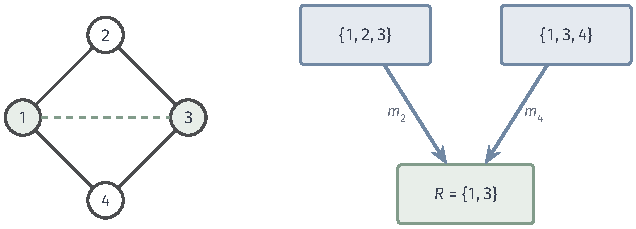
\includegraphics[width=107.500mm]{figures/03-graphs/04-local-functions-and-dynamic-programming/tikz/dp-retained-query/figure.pdf}
  \caption{四环上保留$R=\{1,3\}$的查询结构。左图的绿色虚线是为使保留集成团而补入的结构边，不增加局部成本；右图的两个子袋分别消去$x_2,x_4$，消息在根袋按同一组$(x_1,x_3)$相加。根袋恰为$R$，因此不再取最小。}
  \label{fig:graph-dp-retained-query}
\end{figure}

两个子节点的消息为
\[
\begin{aligned}
m_2(x_1,x_3)&=\min_{x_2}\bigl[\phi_{1,2}(x_1,x_2)+\phi_{2,3}(x_2,x_3)\bigr],\\
m_4(x_1,x_3)&=\min_{x_4}\bigl[\phi_{3,4}(x_3,x_4)+\phi_{1,4}(x_1,x_4)\bigr].
\end{aligned}
\]
根袋就是$R$，不再取最小，$F_R=m_2+m_4$。表~\ref{tab:graph-dp-four-cycle-retained}列出了各候选、回溯表与结果。

\begin{table}[!htb]
  \centering
  \small
  \begin{tabular}{@{}cccccccc@{}}
    \toprule
    $(x_1,x_3)$ & $m_2$的候选 & $m_2$ & $b_2$ & $m_4$的候选 & $m_4$ & $b_4$ & $F_R$及条件最优配置\\
    \midrule
    $(0,0)$ & $4,\ 1$ & $1$ & $1$ & $3,\ +\infty$ & $3$ & $0$ & $4$，$(0,1,0,0)$\\
    $(0,1)$ & $6,\ 1$ & $1$ & $1$ & $3,\ +\infty$ & $3$ & $0$ & $4$，$(0,1,1,0)$\\
    $(1,0)$ & $2,\ 3$ & $2$ & $0$ & $3,\ 1$ & $1$ & $1$ & $3$，$(1,0,0,1)$\\
    $(1,1)$ & $4,\ 3$ & $3$ & $1$ & $3,\ +\infty$ & $3$ & $0$ & $6$，$(1,1,1,0)$\\
    \bottomrule
  \end{tabular}
  \caption{四环算例在$R=\{1,3\}$上的条件最小成本表。“候选”依次对应内部变量取$0,1$；$b_2$、$b_4$是达到最小值的$x_2$、$x_4$；最后一列是由回溯表恢复的条件最优配置。}
  \label{tab:graph-dp-four-cycle-retained}
\end{table}

逐项用表~\ref{tab:graph-dp-four-cycle-enumeration}核对：
\begin{itemize}
  \item $x_1=0,x_3=0$的四个配置成本为$7,+\infty,4,+\infty$，最小$4$在$(0,1,0,0)$；
  \item $x_1=0,x_3=1$的四个为$9,+\infty,4,+\infty$，最小$4$在$(0,1,1,0)$；
  \item $x_1=1,x_3=0$的四个为$5,3,6,4$，最小$3$在$(1,0,0,1)$；
  \item $x_1=1,x_3=1$的四个为$7,+\infty,6,+\infty$，最小$6$在$(1,1,1,0)$。
\end{itemize}
四个表项及条件最优配置都与表中一致。

对整张表取最小，得到
\[
\min(4,4,3,6)=3,
\]
在$(x_1,x_3)=(1,0)$处达到，相应的条件最优配置$(1,0,0,1)$就是第~\ref{sec:graph-dp-four-cycle-min}小节的整体最优配置，两种计算互相印证。

这个查询不能直接用分解$\{1,2,4\}-\{2,3,4\}$回答：那里没有袋同时含$x_1$和$x_3$，$x_1$会在叶节点被取最小。

\paragraph{两个边界}
$R=\varnothing$时不保留变量，查询结构就是原来的结构，表只有一项，计算退化为第~\ref{sec:graph-dp-min-cost}节，四环上为$F^\star=3$。$R=V$时不消去任何变量：补边后的图是完全图，根袋包含全部变量，$F_R=g_r$就是把全部局部项相加的$16$项表，即表~\ref{tab:graph-dp-four-cycle-enumeration}本身。前者不保留任何变量，后者不消去任何变量，一般的查询介于二者之间，输出表的大小与根袋的宽度也随之介于二者之间。

% 第13章第4节：计数和求和（可行配置计数、求和、无保留变量时的汇总、保留变量的累计表、计算正确性、求和与取最小的顺序、四环算例与结果检验）。

\section{计数和求和}
\label{sec:graph-dp-semiring}
\label{sec:graph-dp-counting-sums}

最小成本只关心最好的一个配置。另一类问题要对全部配置汇总：可行配置有多少个，或者按局部权重之积给每个配置一个权重，全部权重加起来是多少。本节先用约束指示函数计算可行配置数，再把指示值推广为非负有限权重。两种计算都把“局部项相加、对变量取最小”换成“局部值相乘、对变量求和”，结构、归属和处理次序都不变；变化在于数值的组合与汇总方式，以及输出的含义。

\subsection{可行配置计数}
\label{sec:graph-dp-feasible-count}

把每个局部函数换成它的可行性指示
\[
\iota_a(\bm x_{S_a})=\begin{cases}1,&\phi_a(\bm x_{S_a})<+\infty,\\0,&\phi_a(\bm x_{S_a})=+\infty.\end{cases}
\]
一个配置可行，当且仅当这些指示全为$1$，即它们的乘积为$1$。于是可行配置数为
\begin{equation}
N=\sum_{\bm x\in\mathcal X}\ \prod_{a\in A}\iota_a(\bm x_{S_a}).
\label{eq:graph-dp-feasible-count}
\end{equation}
输入与最小成本问题相同（只用到哪些组合被禁止），输出是一个非负整数。

在袋树上计算时，节点$u$先把归入它的指示值与子节点交来的计数相乘，
\begin{equation}
h_u(\bm x_{B_u})=\prod_{a\in A_u}\iota_a(\bm x_{S_a})\cdot\prod_{c\in\operatorname{ch}(u)}n_{c\to u}(\bm x_{S_c}),
\label{eq:graph-dp-count-merge}
\end{equation}
再对接口外的状态求和，得到发往父节点的计数消息
\begin{equation}
n_{u\to p(u)}(\bm x_{S_u})=\sum_{\bm x_{I_u}}h_u(\bm x_{S_u},\bm x_{I_u}).
\label{eq:graph-dp-count-message}
\end{equation}
它的含义是：接口取这组值时，$u$下方的变量有多少种取值能使下方全部约束满足。

两种空运算的约定与最小成本不同：空乘积取$1$，求和从$0$开始。没有局部项归入、也没有子节点的袋，$h_u\equiv1$，但求和仍要累计内部变量的全部状态。孤立变量$x_v$单独成袋$\{v\}$时，消息是$\sum_{x_v}1=|\mathcal X_v|$，不能直接把它的计数设为$1$：它不受约束，每个状态都与其余变量的每个可行取值组合成不同的可行配置。

\subsection{求和}
\label{sec:graph-dp-weighted-sum}

把指示值推广为非负有限的局部权重$w_a(\bm x_{S_a})\geq0$，配置的权重定义为各局部权重之积
\[
W(\bm x)=\prod_{a\in A}w_a(\bm x_{S_a}),
\]
要求的是全部配置的权重总和
\begin{equation}
Z=\sum_{\bm x\in\mathcal X}\ \prod_{a\in A}w_a(\bm x_{S_a}).
\label{eq:graph-dp-weighted-sum}
\end{equation}
可行配置计数是取$w_a=\iota_a$的特例。

袋树上的计算与计数相同，只是把指示值换成权重。把本袋权重与子消息的乘积记为
\[
h_u(\bm x_{B_u})=\prod_{a\in A_u}w_a(\bm x_{S_a})\cdot\prod_{c\in\operatorname{ch}(u)}z_{c\to u}(\bm x_{S_c}),
\]
再对接口外状态求和，得到消息
\begin{equation}
z_{u\to p(u)}(\bm x_{S_u})=\sum_{\bm x_{I_u}}h_u(\bm x_{B_u});
\label{eq:graph-dp-sum-message}
\end{equation}
若没有接口外变量，就直接把这个乘积作为消息。

消息表照样以接口为索引，但不再需要回溯表：计数和加权总和是对全部配置的汇总，没有“达到它的配置”。

链上这一递推就是矩阵乘法。把$z_{k-1\to k}$看作行向量，把成对权重看作矩阵，矩阵的元素是$w_{k-1,k}(x_{k-1},x_k)$。于是求和
\[
\sum_{x_{k-1}}z_{k-1\to k}(x_{k-1})\,w_{k-1,k}(x_{k-1},x_k)
\]
正是行向量右乘矩阵。一般袋上对多个变量相乘再求和，则是沿指定轴汇总的张量运算。这些运算可参考\BookChapterRef{chap:linear-operations}{卷二“向量、矩阵与张量的运算”章}。

\subsection{无保留变量时的计数与求和汇总}
\label{sec:graph-dp-total-aggregation}

不保留变量时，根$r$合并得到$h_r$，再对根袋的全部状态求和：
\begin{equation}
Z=\sum_{\bm x_{B_r}}h_r(\bm x_{B_r}),
\label{eq:graph-dp-root-sum}
\end{equation}
输出一个总计数或加权总和。根袋没有变量时（例如只用来连接各分量的空袋），直接取它的合并值。

原始图不连通时，各分量的根经空接口交来标量，即各分量的总计数或总和；空接口意味着结果是单表项标量，但发出它的节点仍须对自己袋中的状态求和。这些标量作为因子乘进根的合并值，所以非连通分量的结果相乘。这与有限集合的乘法原理一致：各分量的取值互相独立地组合。

\paragraph{三元作用域例子}
表~\ref{tab:graph-dp-weights}给出三元作用域例子的权重表，权重恰在禁止的组合处为$0$。在分解$\{1,2,3\}-\{2,3,4\}$上，表~\ref{tab:graph-dp-three-aggregations}对接口的每种取值并列三种任务的左袋消息和右袋汇总值，最后一行是根处的结果：最小成本为$0$，可行配置有$10$个，权重总和为$19$。逐一枚举$16$个配置可以核对这三个数，其中最小成本和可行配置数已在第~\ref{sec:graph-dp-problem}小节的枚举中得到。

\begin{table}[!htb]
  \centering
  \caption{三元作用域例子的非负局部权重。第一列的三位二进制串对$w_A$表示$(x_1,x_2,x_3)$，对$w_B$表示$(x_2,x_3,x_4)$；权重为$0$的位置恰是表~\ref{tab:graph-dp-ternary-tables}中成本为$+\infty$的位置。}
  \label{tab:graph-dp-weights}
  \begin{tabular}{ccccccccc}
    \toprule
    取值 & $000$ & $001$ & $010$ & $011$ & $100$ & $101$ & $110$ & $111$\\
    \midrule
    $w_A$ & $1$ & $2$ & $1$ & $0$ & $2$ & $1$ & $1$ & $1$\\
    $w_B$ & $1$ & $1$ & $2$ & $0$ & $0$ & $2$ & $1$ & $2$\\
    \bottomrule
  \end{tabular}
\end{table}

\begin{table}[!htb]
  \centering
  \caption{三种任务在同一接口上的消息。最小成本使用$\min$与$+$，可行计数与加权总和使用$\sum$与$\times$。“左”列是从$\{1,2,3\}$发出的消息，对$x_1$汇总；“右”列是根袋$\{2,3,4\}$对$x_4$的汇总；根处对每个接口取值组合两列（最小成本相加，其余相乘），再对接口汇总（最小成本取最小，其余求和）。}
  \label{tab:graph-dp-three-aggregations}
  \begin{tabular}{ccccccc}
    \toprule
    & \multicolumn{2}{c}{最小成本} & \multicolumn{2}{c}{可行计数} & \multicolumn{2}{c}{加权总和}\\
    \cmidrule(lr){2-3}\cmidrule(lr){4-5}\cmidrule(lr){6-7}
    $(x_2,x_3)$ & 左 & 右 & 左 & 右 & 左 & 右\\
    \midrule
    $(0,0)$ & $0$ & $1$ & $2$ & $2$ & $3$ & $2$\\
    $(0,1)$ & $0$ & $0$ & $2$ & $1$ & $3$ & $2$\\
    $(1,0)$ & $1$ & $0$ & $2$ & $1$ & $2$ & $2$\\
    $(1,1)$ & $2$ & $1$ & $1$ & $2$ & $1$ & $3$\\
    \midrule
    根处 & \multicolumn{2}{c}{$\min(1,0,1,3)=0$} & \multicolumn{2}{c}{$4+2+2+2=10$} & \multicolumn{2}{c}{$6+6+4+3=19$}\\
    \bottomrule
  \end{tabular}
\end{table}

以接口取$(1,1)$的一行为例：$x_1=0$的一行被禁止，左袋的最小成本消息为$\min(+\infty,2)=2$，计数消息为$0+1=1$，加权消息为$0+1=1$。三种任务的计算量与表大小相同，但输出含义不同：最小成本是一个配置的值，可以回溯出达到它的配置；计数和加权总和是对全部配置的汇总。

\subsection{保留变量的累计表}
\label{sec:graph-dp-retained-aggregation}

给定保留集$R$，使用根袋覆盖$R$的查询结构（第~\ref{sec:graph-dp-query-assignment}小节），非根节点照常计算，根处只对$B_r\setminus R$求和：
\begin{equation}
Z_R(\bm x_R)=\sum_{\bm x_{B_r\setminus R}}h_r(\bm x_{B_r}).
\label{eq:graph-dp-retained-sum}
\end{equation}
结果以$\bm x_R$为索引，逐项表示把$R$固定成这组值时的可行配置数（指示权重）或权重总和。再对所有$\bm x_R$求和，才得到第~\ref{sec:graph-dp-total-aggregation}小节的总量$Z$。

与条件最小成本表相比，累计表的每一项不是一个配置的值，而是一组配置的累计；它也不需要回溯表。不含$R$的分量交来的标量作为因子乘到表的每一项上。

\subsection{计算正确性}
\label{sec:graph-dp-sum-correctness}

\paragraph{求和的三条规则}
最小成本递推所用的三条最小值规则，在求和与相乘下有完全对应的形式。设$y,z$在有限集合中取值，$h,g$取非负有限值，$c$与$y$无关，则
\[
\sum_{y,z}h(y,z)=\sum_z\sum_y h(y,z),\qquad \sum_y c\,g(y)=c\sum_y g(y),
\]
并且对取值于互不相交变量组$y_1,\ldots,y_k$的函数，
\[
\sum_{y_1,\ldots,y_k}\prod_j g_j(y_j)=\prod_j\sum_{y_j}g_j(y_j).
\]
第一条是有限求和的重排；第二条是乘法对加法的分配律；第三条由分配律展开乘积得到，展开后的每一项恰对应各$y_j$的一组取值。

\paragraph{消息的含义}
仿照定理~\ref{thm:graph-dp-bag-message}，记号同前，求和任务的消息满足
\[
z_{u\to p(u)}(\bm x_{S_u})=\sum_{\bm x_{V_{D_u}\setminus S_u}}\ \prod_{a\in A_{D_u}}w_a(\bm x_{S_a}),
\]
并且$Z=\sum_{\bm x_{B_r}}h_r(\bm x_{B_r})$。证明逐字沿用那里的拆分：变量集合$I_u$与各$V_{D_{c_j}}\setminus B_u$两两不交，并恰好组成$V_{D_u}\setminus S_u$；固定$\bm x_{B_u}$后，各子树的乘积只依赖互不相交的变量组，由第三条规则分别求和，由归纳假设得到各子消息；归入$u$的权重由第二条规则提到求和号外；最后由第一条规则对$\bm x_{I_u}$求和。

这一论证同时说明每个配置恰被累计一次。下方变量的每一组取值，唯一地分解为内部变量的一组取值和各子树中变量的一组取值；分配律展开后，每组取值恰好贡献一个乘积项$\prod_{a\in A_{D_u}}w_a$。取指示权重时，这个乘积是$1$或$0$，消息就是可行取值的个数，根处给出可行配置数。

逐项固定保留变量，同样的论证给出累计表~\eqref{eq:graph-dp-retained-sum}的正确性，全表求和得到总量。固定输入、保留集和输出要求后，仅改变待求和变量的消去次序不改变结果，因为有限求和可以任意重排；定理~\ref{thm:graph-dp-elimination-equals-messages}的对应关系也照样成立。

\paragraph{共同的代数结构}
三种任务共用同一套递推，是因为它们的运算满足同样的代数规则。每种任务都用到两种运算，分工不同：一种把同一配置的各局部项组合成这个配置的值（相加或相乘），另一种把不同取值的结果汇总成一个数（取最小或全部加起来）。消息之所以能在局部提前汇总，靠的是“先组合再汇总”与“先汇总再组合”结果相同，例如$a+\min(b,c)=\min(a+b,a+c)$、$a(b+c)=ab+ac$：与被汇总变量无关的项$a$可以留到汇总之后再组合。

把这些规则抽象出来。设集合$\mathcal S$上有两种运算：$\oplus$用于跨不同取值的汇总，$\otimes$用于在一个配置内组合各局部项。若两种运算都满足结合律和交换律，各有单位元$\bar0$与$\bar1$，满足$\bar0\otimes a=\bar0$，并且$\otimes$对$\oplus$满足分配律
\[
a\otimes(b\oplus c)=(a\otimes b)\oplus(a\otimes c),
\]
就称$(\mathcal S,\allowbreak\oplus,\allowbreak\otimes,\allowbreak\bar0,\allowbreak\bar1)$为交换\term{半环}（semiring）。

最小成本对应$(\mathbb R\cup\{+\infty\},\allowbreak\min,\allowbreak+,\allowbreak+\infty,\allowbreak0)$，此时分配律就是$a+\min(b,c)=\min(a+b,a+c)$；计数对应自然数上的$(+,\times,0,1)$；加权求和对应非负实数上的$(+,\times,0,1)$；只判断是否存在可行配置时，还可以用布尔值上的“或”与“且”。

把变量消元和袋消息中的$\min$换成$\oplus$、$+$换成$\otimes$，前面的正确性证明逐字成立，因为证明只用到了结合律、交换律和分配律。半环不要求减法或除法。

\subsection{求和与取最小的顺序}
\label{sec:graph-dp-mixed-order}

上面的换序结论只针对同一种汇总：纯最小化中可以任意交换取最小的次序，纯求和中可以任意交换求和的次序。把本节的求和与第~\ref{sec:graph-dp-min-cost}节的取最小放在一起，情况就不同了。

取一张两行两列的成本表$h(y,z)$，两行分别为$(0,1)$与$(1,0)$，即$h(0,0)=h(1,1)=0$、$h(0,1)=h(1,0)=1$。每行先对$z$求和得$1$与$1$，再对两行取最小，得到
\[
\min_y\sum_z h(y,z)=\min(1,1)=1 .
\]
反过来先对每一列在两行之间取最小，两列都得到$0$，再求和，得到
\[
\sum_z\min_y h(y,z)=0+0=0 .
\]
前者要求所有$z$共用同一个$y$，后者允许$y$随$z$改变，所以两种顺序回答的是不同的问题。

\paragraph{混合汇总}
不同变量混合使用求和与取最小（或取最大）时，须按所求结果确定运算顺序，不能直接沿用纯求和或纯最小化的换序结论。例如对表$h(x,y)$，$h(0,0)=h(1,1)=4$、$h(0,1)=h(1,0)=0$，有
\[
\max_x\sum_y h(x,y)=4,\qquad \sum_y\max_x h(x,y)=8 .
\]
这类混合问题只能按限定的次序消元：被外层汇总的变量必须最后处理，消元次序因而受到约束，所需的中间表可能比单一汇总时大。把非负权重归一化为概率还要求总和为正且有限；这些概率解释、边缘化查询以及带环图上的近似消息方法，都留到后续的概率推断内容。

\subsection{四环算例与结果检验}
\label{sec:graph-dp-four-cycle-sums}

\paragraph{约束指示表与权重表}
四环算例的约束指示表由表~\ref{tab:graph-dp-four-cycle-costs}读出：只有$\iota_{3,4}(1,1)=0$与$\iota_{1,4}(0,1)=0$，其余指示值都是$1$。另取一组非负权重，在被禁止的组合处为$0$，其余取$1$或$2$，见表~\ref{tab:graph-dp-four-cycle-weights}；这些权重是教学示例，与成本表的具体数值无关。

\begin{table}[!htb]
  \centering
  \caption{四环算例的非负局部权重。行列约定与表~\ref{tab:graph-dp-four-cycle-costs}相同；权重为$0$的位置恰是成本为$+\infty$的位置。}
  \label{tab:graph-dp-four-cycle-weights}
  \begin{tabular}{cccc}
    \toprule
    $w_{1,2}(x_1,x_2)$ & $w_{2,3}(x_2,x_3)$ & $w_{3,4}(x_3,x_4)$ & $w_{1,4}(x_1,x_4)$\\
    \midrule
    $\begin{bmatrix}1&2\\2&1\end{bmatrix}$ &
    $\begin{bmatrix}2&1\\1&1\end{bmatrix}$ &
    $\begin{bmatrix}1&2\\1&0\end{bmatrix}$ &
    $\begin{bmatrix}1&0\\1&2\end{bmatrix}$\\
    \bottomrule
  \end{tabular}
\end{table}

\paragraph{总量}
在分解$\{1,2,4\}-\{2,3,4\}$上以$\{2,3,4\}$为根。叶节点对$x_1$求和：计数消息为
\[
n(x_2,x_4)=\sum_{x_1}\iota_{1,2}\,\iota_{1,4}=(2,\ 1,\ 2,\ 1),
\]
加权消息为
\[
\begin{aligned}
z(x_2,x_4)&=\sum_{x_1}w_{1,2}\,w_{1,4}\\
&=(1\cdot1+2\cdot1,\ 1\cdot0+2\cdot2,\ 2\cdot1+1\cdot1,\ 2\cdot0+1\cdot2)\\
&=(3,4,3,2),
\end{aligned}
\]
取值按$(x_2,x_4)$的字典序排列。

根处把消息与$\phi_{2,3},\phi_{3,4}$对应的指示值或权重相乘，按$(x_2,x_3,x_4)$的字典序，计数的合并值为
\[
(2,1,2,0,2,1,2,0),
\]
求和得$N=10$。加权的合并值为
\[
(6,16,3,0,3,4,3,0),
\]
求和得$Z=35$。

用表~\ref{tab:graph-dp-four-cycle-enumeration}核对：可行配置恰有$10$个。逐个计算可行配置的权重，按字典序依次为$2,1,2,2,4,16,2,1,4,1$，总和为$35$。例如最优配置$(1,0,0,1)$的权重为
\[
w_{1,2}(1,0)\,w_{2,3}(0,0)\,w_{3,4}(0,1)\,w_{1,4}(1,1)=2\cdot2\cdot2\cdot2=16.
\]

\paragraph{保留变量的累计表}
在$R=\{1,3\}$的查询结构上，两个子节点分别对$x_2$与$x_4$求和，根袋$\{1,3\}$把两条消息相乘，不再求和。按$(x_1,x_3)$的字典序，计数消息为$(2,2,2,2)$与$(1,1,2,1)$，累计表为
\[
N_R=(2,\ 2,\ 4,\ 2);
\]
加权消息为$(4,3,5,3)$与$(1,1,5,1)$，累计表为
\[
Z_R=(4,\ 3,\ 25,\ 3).
\]
全表求和分别为
\[
2+2+4+2=10=N,\qquad 4+3+25+3=35=Z.
\]

下面逐项核对。例如$x_1=1,x_3=0$时，可行配置为
\[
 (1,0,0,0),\qquad (1,0,0,1),\qquad (1,1,0,0),\qquad (1,1,0,1),
\]
共$4$个，权重之和为$4+16+1+4=25$。

\paragraph{结果的解释与边界}
计数为零表示没有可行配置：第~\ref{sec:graph-dp-four-cycle-min}小节的不可行约束变体中，叶节点的计数消息为$(0,1,1,0)$，根处要求$x_2=x_3=x_4$时这条消息为$0$，于是$N=0$，与最小成本为$+\infty$一致。

一般的加权和为零却不直接表示不可行：权重可以在可行的组合上取$0$，例如把$w_{1,2}$全部改为$0$，则$Z=0$，而可行配置仍有$10$个。

第~\ref{sec:graph-dp-four-cycle-min}小节加入孤立变量$x_5\in\{0,1,2\}$和边$\{6,7\}$后，两个新分量经空接口交来标量。袋$\{5\}$没有局部项，$h\equiv1$，计数消息为$3$。若$\phi_{6,7}$的四项都有限，袋$\{6,7\}$的计数消息为$4$；若再给它权重表
\[
w_{6,7}=\begin{bmatrix}1&1\\2&1\end{bmatrix},
\]
加权消息为$5$。根把这些标量乘进合并值，得
\[
N=10\cdot3\cdot4=120,\qquad Z=35\cdot3\cdot5=525.
\]若错把孤立变量的计数设为$1$，结果会少乘一个因子$3$。

% 第13章第5节：计算代价（状态表的规模、时间代价、存储代价、时间与存储的取舍）。

\section{计算代价}
\label{sec:graph-dp-computation-cost}

前几节的计算都给出精确结果，但所需的时间和存储可能很大。本节把已构建的袋和接口换算成实际的状态组合数，分别分析求值的时间、存储及二者的取舍。结构的构造方法见第~\ref{sec:graph-tree-decomposition-construction}节；这里给出的资源指标可以用来比较不同的构造结果，构造与核验本身的成本也一并计入任务的总成本。

\subsection{状态表的规模}
\label{sec:graph-dp-table-size}

先固定规模变量：变量个数$n$，局部项个数$|A|$，袋树节点数$N$，第$i$个变量的状态数$|\mathcal X_i|$，以及$q=\max_i|\mathcal X_i|$。对一组变量$U$，记它上面的配置数为
\[
|\mathcal X_U|=\prod_{i\in U}|\mathcal X_i| .
\]
计算中出现三类表：袋$u$上的合并表有$|\mathcal X_{B_u}|$项，接口消息和回溯表各有$|\mathcal X_{S_u}|$项（回溯表的每一项存$|I_u|$个变量的取值），保留变量的输出表有$|\mathcal X_R|$项。

在每个变量至多$q$个状态、分解宽度为$w$时，每个袋至多$w+1$个变量，袋表至多$q^{w+1}$项。但这只是上界：接口与输出仍按实际变量计算，状态数不同的变量对乘积的贡献也不同。比较两个候选结构时，应固定同一任务（同一保留集、同一输出要求），并使用实际的乘积，而不是只比较宽度。例如两个结构宽度都是$2$，一个的最大袋由三个二值变量组成（$8$项），另一个含一个十状态变量（至少$40$项），实际规模相差数倍。

图~\ref{fig:graph-dp-table-size}把这个差别落实为表项：两侧都只有三个变量，但十状态变量需要十组而不是两组配置。同为宽度$2$，并不意味着同样的读表和存储代价。

\begin{figure}[!htb]
  \centering
  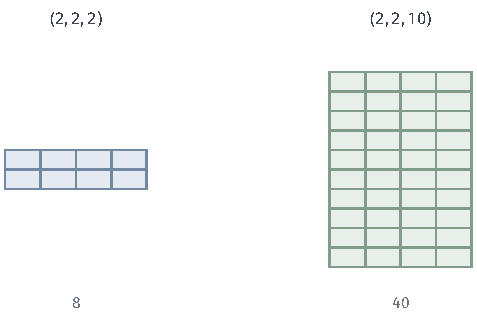
\includegraphics[width=80.617mm]{figures/03-graphs/04-local-functions-and-dynamic-programming/tikz/dp-table-size/figure.pdf}
  \caption{相同袋宽度下的实际表规模。括号给出三个变量各自的状态数，每格对应一种联合取值。左表为$2\times2\times2=8$项，右表为$2\times2\times10=40$项；四列枚举前两个二值变量，行枚举第三个变量。}
  \label{fig:graph-dp-table-size}
\end{figure}

宽度出现在指数上，这是精确计算的主要限制。$q=10$、$w=10$时一张袋表就有$10^{11}$项；若查询要求保留很多变量的联合表，输出本身也可能大得不可承受，这时任何精确方法都必须至少写出整张表。

四环算例中，分解$\{1,2,4\}-\{2,3,4\}$的两个袋各有$8$项，接口消息和回溯表各有$4$项；$R=\{1,3\}$的查询结构有两个$8$项的袋、一个$4$项的根袋，输出表$4$项。按次序$(1,2,3,4)$不合并时，四个消元簇的配置数为$8,8,4,2$。

\subsection{时间代价}
\label{sec:graph-dp-time-cost}

约定表查询、加法、乘法和比较各计一次基本运算。处理节点$u$时，要对$\bm x_{B_u}$的每种取值读取归入$u$的每个局部项一次、读取每条子消息一次，把它们组合起来，再参与一次取最小或求和，所以工作量约为
\[
|\mathcal X_{B_u}|\,\bigl(|A_u|+|\operatorname{ch}(u)|+1\bigr).
\]
对全部节点求和，利用袋树中$\sum_u|\operatorname{ch}(u)|=N-1$，求值时间为
\[
\sum_{u}|\mathcal X_{B_u}|\,\bigl(|A_u|+|\operatorname{ch}(u)|+1\bigr)=O\bigl((|A|+N)\,q^{w+1}\bigr).
\]
可见单个袋表的上界$q^{w+1}$还要乘以袋数和每项的工作量，才给出总时间。

按消元次序计算时，消去$x_i$要对$\{i\}\cup S_i$的至多$q^{|S_i|+1}$种取值各读取$\mathcal F_i$中每个函数一次，时间约为
\[
|\mathcal F_i|\,q^{|S_i|+1}.
\]
每个函数恰好在它的某个变量被消去时被取出一次，原有函数$|A|$个，新函数至多$n$个，所以各步的$|\mathcal F_i|$之和不超过$|A|+n$；按变量维护索引的开销也与函数个数成正比。若诱导宽度为$w$，总时间为
\[
O\bigl((|A|+n)\,q^{w+1}\bigr),
\]
而枚举为$|A|\,q^n$。

除向上的求值外，还要计入结果输出与配置恢复。条件最小成本表或累计表的输出要写出$|\mathcal X_R|$项。恢复一个配置时每个节点只查一次回溯表，共$O\bigl(\sum_u|B_u|\bigr)$次读写，与求值相比可以忽略。若还需要每个袋上各取值的最小总成本，就像第~\ref{sec:graph-dp-tree-two-pass}小节那样再按前序发送一遍反向消息，时间约加倍。

结构构造与核验的时间单独计算，再加入任务的总时间：模拟消元为$O\bigl(n+m+\sum_t d_t^2\bigr)$（第~\ref{sec:graph-dp-clusters-to-decomposition}小节），检验为袋大小的多项式（第~\ref{sec:graph-dp-construction-check}小节）。同一结构用于多组数值时，这部分只付一次。

计数中的整数加乘在上面各计一次基本运算。若要考虑位复杂度，还须按数值的位数分析：可行配置数至多为$\prod_i|\mathcal X_i|\leq q^n$，需要约$n\log_2q$位，大规模问题中一次加乘的实际代价随位数增长；加权求和若用浮点数，还要另行分析舍入误差。

\subsection{存储代价}
\label{sec:graph-dp-memory-cost}

存储要分清对象，并按计算过程中同时保留的对象计算峰值，不能把累计生成的表项总量或单个接口的规模直接当作峰值。计算中要存放的对象有四类：
\begin{itemize}
  \item 接口消息：每张$|\mathcal X_{S_u}|$项，从生成起保留到父节点用完为止；
  \item 临时袋表：处理节点$u$时的合并表，若整张存放有$|\mathcal X_{B_u}|$项；
  \item 达到值记录：每个非根节点一张回溯表，$|\mathcal X_{S_u}|$项，每项存$|I_u|$个取值，要保留到恢复结束；
  \item 输出表：保留变量查询的$|\mathcal X_R|$项。
\end{itemize}

临时袋表不必整张存放。对接口的每个取值，可以逐个枚举内部变量的取值，现场计算$g_u$的一项并立即并入当前的最小值（或累加和），算完一个接口取值就写出消息的一项。这样处理节点$u$时只需$O(|B_u|)$的工作空间，而不是$|\mathcal X_{B_u}|$；代价是对局部项和子消息的读取顺序不再连续，常数因子可能变大。

消息的保留时间取决于后序。只求最优值而不恢复配置时，子节点的消息在父节点处理完后即可释放，所以任一时刻保留的只是“已处理完、父节点尚未处理”的那些节点的消息。链状袋树上同时只有一条消息；一个根下挂很多叶节点时，处理根之前全部叶节点的消息同时存在。峰值是这些同时存在的消息之和，加上当前节点的工作空间，而不是全部消息的总和。

图~\ref{fig:graph-dp-message-frontier}对比了两种后序计算的中间时刻。只需最优值、并在父节点使用后释放子消息时，链上只留下最近生成的一条消息；星形结构在处理根之前则须同时保存各叶节点的消息。

\begin{figure}[!htb]
  \centering
  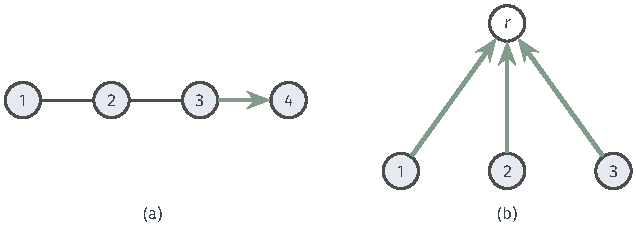
\includegraphics[width=107.500mm]{figures/03-graphs/04-local-functions-and-dynamic-programming/tikz/dp-message-frontier/figure.pdf}
  \caption{同时存活的消息决定峰值存储。圆点表示袋，绿色箭头表示已经生成、仍待父袋读取的消息。(a)链上袋$1,2$的消息已被后继使用并释放，仅袋$3$的消息仍在；(b)根$r$尚未处理，三个叶袋的消息同时存在。此处比较消息存储，不包含回溯表或输出表。}
  \label{fig:graph-dp-message-frontier}
\end{figure}

需要恢复配置时，回溯表要保留到前序回溯走完，存储为$\sum_u|\mathcal X_{S_u}|\cdot|I_u|$量级，这时可以释放的只有消息。

四环算例中，最小成本计算的峰值是一条$4$项消息加根处的工作空间；恢复配置还要保留一张$4$项的回溯表。$R=\{1,3\}$的查询中，处理根之前两条$4$项消息同时存在，输出表另有$4$项。

\subsection{时间与存储的取舍}
\label{sec:graph-dp-time-memory-tradeoff}

固定同一结构和输出要求，可以在三种做法之间取舍：缓存中间结果、在最后一次使用后释放、或者按需重算。

最直接的是全部缓存：保留所有消息和回溯表，向上一遍后既能恢复配置，也能再发一遍反向消息得到每个袋的表，时间最少，存储最多。只需最优值时，在最后一次使用后立即释放消息，存储降到上一小节的峰值，时间不变。

回溯表也可以不存。若保留各条子消息，恢复时对每个节点$u$在已知接口取值下重新枚举$\bm x_{I_u}$、重算$g_u$并取最小点，就能得到与回溯表相同的选择（并列规则保持一致即可）；额外时间是每个节点$|\mathcal X_{I_u}|$量级的重算，存储从回溯表换成消息。若连消息也释放了，恢复时就要重新计算子树的消息，时间可能成倍增加。总之，释放后仍要用到的信息只能重算，或者从另存的记录中读回。

是否恢复配置、是否保存整张保留变量表，都会改变记录的保留时机。只要整体最优值时，回溯表根本不必生成；只要条件最小成本表而不要条件最优配置时，根处的回溯表可以省去。

只查询少数几个$\bm x_R$而不是整张表时，可以对每个查询值把$\bm x_R$固定后按第~\ref{sec:graph-dp-min-cost}节计算一次，用查询次数乘以单次时间换取不必存放$|\mathcal X_R|$项的输出表。哪种做法更合适，取决于结构的实际规模和输出要求，应在固定任务后按上面的资源指标比较。

\FloatBarrier
\section{本章小结}
\label{sec:dp-computation-chapter-summary}

本章在已核验的结构上完成数值计算。所有任务共用同一套组织：每个局部项恰好归入一个容纳其作用域的袋，按后序由叶到根处理，每个节点合并本地的局部项与子节点交来的表，对内部变量汇总，把以接口为索引的结果交给父节点。按消元次序计算与沿消元森林计算得到同样的中间函数；合并袋、调整归属或改变同类汇总的次序会改变中间表，不改变最终结果。

最小成本问题同时求值和恢复最优配置：合并用加法，汇总取最小，取最小时记下达到值，根选定最优状态后沿前序查回溯表，等价于按消元的逆序回溯；最小值为$+\infty$时报告不可行，并列最优按固定规则选取。带保留变量时，查询结构使根袋覆盖保留集，保留变量从不在非根节点被汇总，根处只对其余变量取最小，输出各固定配置下的最小成本，并可恢复相应的条件最优解。计数和求和把加法换成乘法、取最小换成求和，消息表示下方的可行取值数或权重总和，非连通分量的结果相乘，孤立变量贡献其状态数；它们不需要回溯表。

正确性都来自同一个不变量：消息等于固定接口后下方全部局部项的最优值或累计值。它依赖三项条件：运行交集使接口隔开两侧，顶点覆盖使根处涉及全部变量，唯一归属使每项只计一次；再加上组合与汇总运算的结合律、交换律和分配律。这些规则只保证同一种汇总可以换序，求和与取最小混用时不能交换，四项小表就给出$1$与$0$两个不同结果。

实际代价由袋、接口、各变量的状态数、输出要求与存储安排共同决定。宽度给出袋表$q^{w+1}$的上界，比较结构时应使用实际的状态数之积；求值时间约为各袋配置数乘以逐项工作量之和，结构构造与核验另计；存储按同时保留的消息、回溯表和输出计算峰值，可以用释放和重算换取存储。四环算例在全部任务上与枚举逐项一致。

至此，本部分从局部函数出发，经链和树上的接口递推、一般图上的结构构建，完成了有限状态配置问题的精确计算。

